\section*{Appendix}
\label{sec:appendix}

\begin{frame}[allowframebreaks]{\nameref{sec:appendix}: Bayesian Lasso}
    \begin{theorem}
        Under a Laplace prior and i.i.d normally distributed errors the posterior mode is the frequentist Lasso estimate.
    \end{theorem}

    The full Bayesian Lasso model can be found in \cite{park_bayesian_2008}.\\~\\

    \textbf{Proof.}\\
    Consider the standard regression model $y_i = \beta_0 + \sum_{j = 1}^{p} \beta_j x_{ij} + \epsilon_i$ with $\epsilon_i \overset{\text{i.i.d.}}{\sim} N(0, \sigma^2)$ and i.i.d. $\beta = \beta_1 , \beta_2 , \dots , \beta_p$ and:

    \begin{itemize}
        \small
        \item Likelihood: $p(y|X,\beta) = \prod_{i = 1}^{n} \frac{1}{\sqrt{2 \pi} \sigma} \exp \left( - \frac{\epsilon_i^2}{2 \sigma^2} \right) \propto \exp \left( - \frac{1}{2 \sigma^2} \sum_{i = 1}^{n} \epsilon_i^2 \right)$ with $\epsilon_i = y_i - \beta_0 - \sum_{j = 1}^{p} \beta_j x_{ij}$
        \item Laplace prior centered at zero: $p(\beta;\tau) = \prod_{j = 1}^{p} \frac{1}{2\tau} \exp \left( - \frac{|\beta_j|}{\tau} \right) \propto \exp \left( - \frac{1}{\tau} \sum_{j = 1}^{p} |\beta_j| \right)$
    \end{itemize}

    The posterior $p(\beta|y,X) \propto p(y|X,\beta) p(\beta;\tau)$ can be written as:

    \begin{align*}
        p(\beta|y,X) & \propto\overbrace{\exp \left( - \frac{1}{2 \sigma^2} \sum_{i = 1}^{n} \epsilon_i^2 \right)}^{\text{Likelihood}} \overbrace{\exp \left( - \frac{1}{\tau} \sum_{j = 1}^{p} |\beta_j| \right)}^{\text{Prior}} \\
                     & = \exp \left( - \frac{1}{2 \sigma^2} \sum_{i = 1}^{n} \epsilon_i^2 - \frac{1}{\tau} \sum_{j = 1}^{p} |\beta_j| \right)
    \end{align*}

    Taking the $\log$ to determine the posterior mode optimization problem:

    \begin{align*}
        \log p(\beta|y,X) & = - \frac{1}{2 \sigma^2} \sum_{i = 1}^{n} \epsilon_i^2 - \frac{1}{\tau} \sum_{j = 1}^{p} |\beta_j| = - \left( \frac{1}{2 \sigma^2} \sum_{i = 1}^{n} \epsilon_i^2 + \frac{1}{\tau} \sum_{j = 1}^{p} |\beta_j| \right)
    \end{align*}

    Maximizing the negative log posterior is equal to minimizing the positive log posterior:

    \begin{align*}
        \text{arg} \min_{\beta} \left[ \frac{1}{2 \sigma^2} \sum_{i = 1}^{n} \epsilon_i^2 + \frac{1}{\tau} \sum_{j = 1}^{p} |\beta_j| \right] = \text{arg} \min_{\beta} \frac{1}{2 \sigma^2} \left[ \sum_{i = 1}^{n} \epsilon_i^2 + \frac{2 \sigma^2}{\tau} \sum_{j = 1}^{p} |\beta_j| \right]
    \end{align*}

    Ignoring the normalizing constant $\frac{1}{2 \sigma^2}$ and setting $\lambda = \frac{2 \sigma^2}{\tau}$ yields the Lasso estimate:
    \begin{align*}
        \text{arg} \min_{\beta} \left[ \sum_{i = 1}^{n} \epsilon_i^2 + \lambda \sum_{j = 1}^{p} |\beta_j| \right]
    \end{align*}

    \hfill$\square$
\end{frame}

\begin{frame}{\nameref{sec:appendix}: Sparsified variance-covariance matrix estimates}
    \begin{figure}
        \centering
        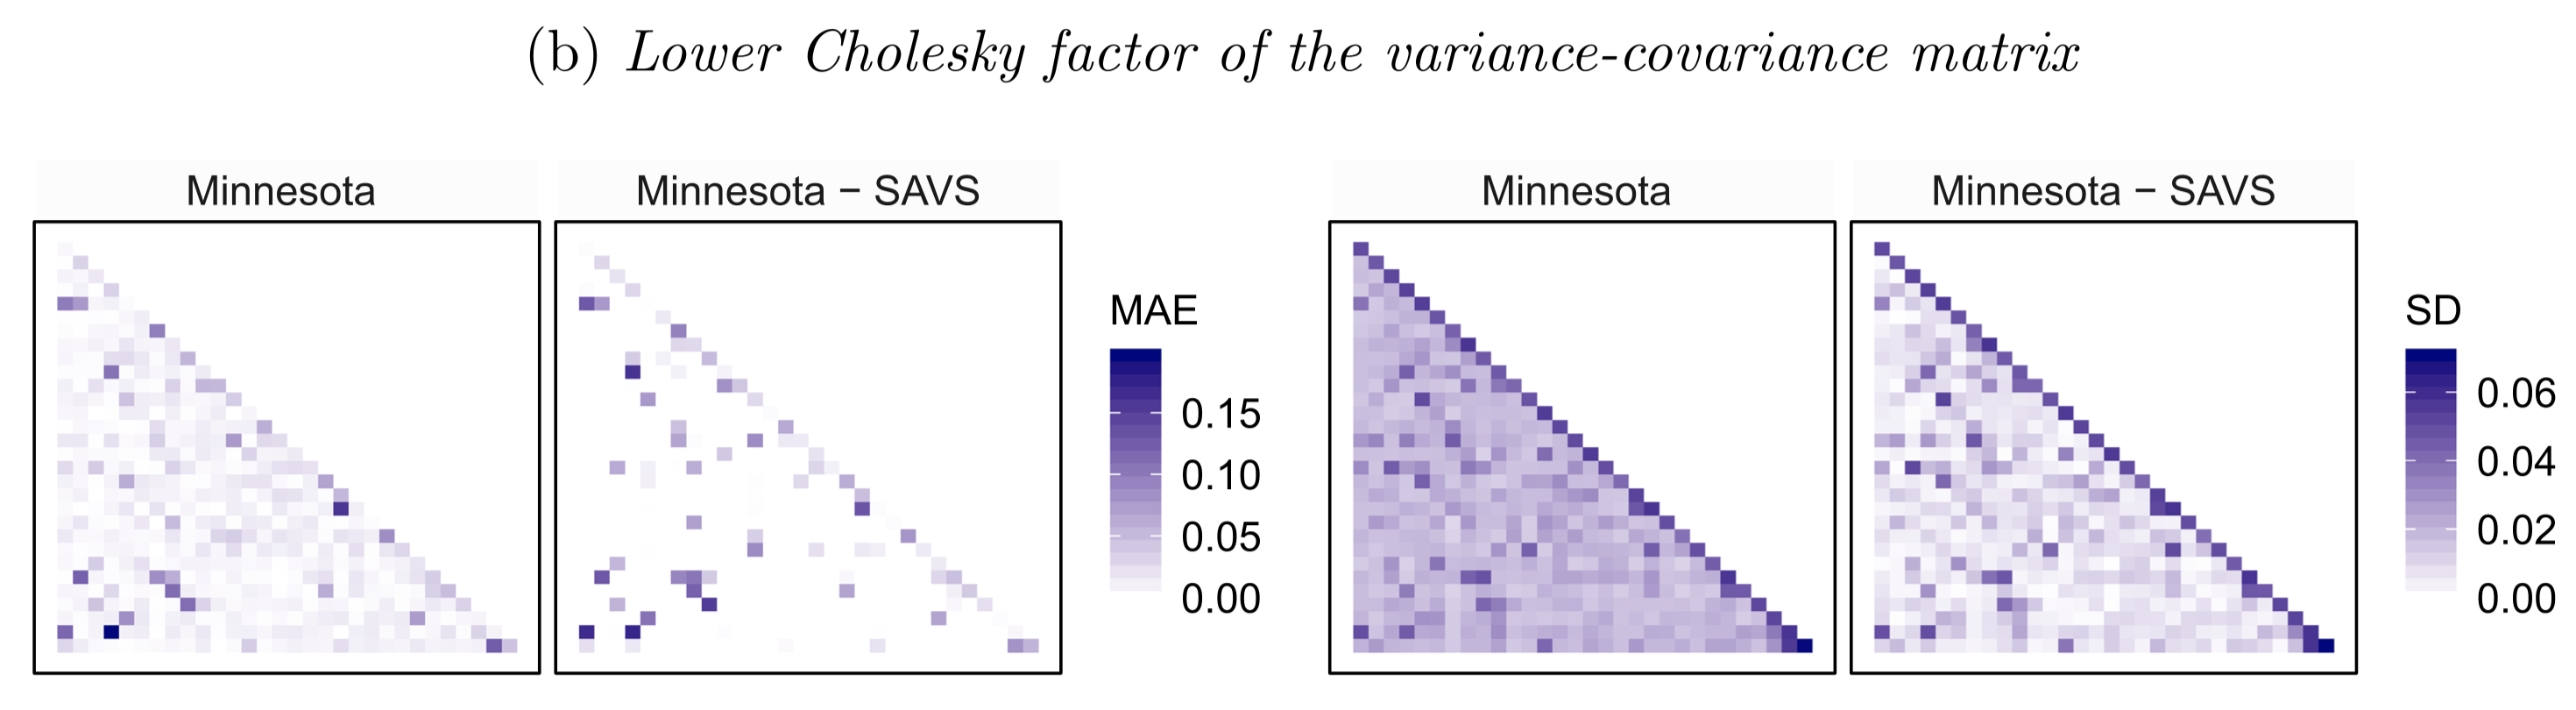
\includegraphics[width=1\textwidth]{plots/sparsity_covariance_matrix.png}
        \caption{Similar to the results in Figure~\ref{fig:dense_vs_sparse_coefficients}, sparsification also reduces the MAE as well as the predictive uncertainty of the variance-covariance matrix estimates.}
        \label{fig:dense_vs_sparse_covariance_matriy}
    \end{figure}
\end{frame}

\begin{frame}{\nameref{sec:appendix}: Root-mean-squared-forecast-error (RMSE)}
    The root-mean-squared-forecast-error (RMSE) describes the square-root of the squared average deviation of forecasts from the true values. It can be written as follows:\footcite{banbura_large_2010}
    
    \begin{align*}
        \text{RMSE} = \sqrt{\frac{1}{T_1 - T_0 - H + 1} \sum_{T = T_0 + H - h}^{T_1 - h} (y_{i , T + h | T} - y_{i , T + h})^2}
    \end{align*}
    
    where $y_{i , T + h | T}$ is the point estimate (e.g. posterior median) at time $T + h$ given the information set for the time span $T$ and $y_{i , T + h}$ the true value at time $T + h$. $T_0$ and $T_1$ are the beginning and the end of the evaluation sample and $H$ the longest forecast horizon.
\end{frame}

\begin{frame}{\nameref{sec:appendix}: Predictive likelihood}
    The predictive likelihood is the posterior predictive density evaluated at the actual true outcome. The sum of log predictive likelihoods can be used to compare the forecasting performance of one model relative to other models. It is defined as follows:\footcite{koop_forecasting_2013}
    
    \begin{align*}
        \sum_{T = T_0}^{T_1 - h} \log [ p(y_{i , T + h | T} = y_{i , T + h} | \text{Data}_T) ]
    \end{align*}
    
    where $y_{i , T + h | T}$ is the point estimate (e.g. posterior median) at time $T + h$ given the information set for the time span $T$ and $y_{i , T + h}$ the true value at time $T + h$. $T_0$ and $T_1$ are the beginning and the end of the evaluation sample and $h$ the forecast horizon. Finally, $\text{Data}_T$ is the information set available at time T. 
\end{frame}
